% !TeX TS-program = xelatex -synctex=1 -interaction=nonstopmode -shell-escape -output-directory=build %.tex
\documentclass[aspectratio=169]{beamer}

% All my packages are specified and set up in include/format:
\usepackage{include/format}

\title{IoT Crashcourse for Begyndere}
\subtitle{Med ESP32}

\author{Jacob Bechmann Pedersen}
\institute{Bechmann Engineering ApS}
\date{\today}

%% Reference settings:
\renewcommand{\figurename}{Figur}
\renewcommand{\tablename}{Tabel}
\renewcommand{\refname}{Referenceliste}
\renewcommand{\contentsname}{Indhold}
\renewcommand{\listfigurename}{Figurliste}
\renewcommand{\listtablename}{Tabelliste}
\renewcommand{\lstlistlistingname}{Kodeliste}

\begin{document}

\begin{frame}
	\titlepage
\end{frame}

\begin{frame}{Indhold}
	\begin{columns}
	\begin{column}{0.6\textwidth}
		\begin{fitBox}
			\tableofcontents{}
		\end{fitBox}
	\end{column}
	\begin{column}{0.4\textwidth}
		\centering
		\begin{figure}
  			\includesvg[height=0.6\textheight]{assets/svg/ESP32-DevkitC-v4.svg}
  			\caption{ESP32 DevkitC v4, boardet vi skal arbejde med}
  			\label{fig:esp32}
		\end{figure}
	\end{column}
	\end{columns}	
\end{frame}

\section{Hvem er jeg?}
\begin{frame}[fragile]{Hvem er jeg?}
\begin{columns}
	\begin{column}{0.4\textwidth}
		\begin{center}
		\roundedGfx{0.8\textwidth}{assets/pictures/portrait.png}
		\vspace{0.05\textwidth}
		\begin{columns}
			\begin{column}{0.33\textwidth}
	  			\roundedGfx{\textwidth}{assets/pictures/shiny-hunter.jpg}
			\end{column}
			\begin{column}{0.33\textwidth}
	  			\roundedGfx{\textwidth}{assets/pictures/hackrf.jpg}
			\end{column}
			\begin{column}{0.33\textwidth}
  				\roundedGfx{\textwidth}{assets/pictures/wifi-picture.jpg}
			\end{column}
		\end{columns}
		\end{center}
	\end{column}	

	\begin{column}{0.6\textwidth}
	\begin{textBox}
		Jacob Bechmann Pedersen
			\begin{itemize}
				\item Kursus-/Foredragsholder om embedded elektronik, programmering og Arduino
				\item Tidl. Embedded electronics engineer hos DTU Elektro, Automation and Control
					\begin{itemize}
						\item Robotter, embedded Linux, autonome systemer
					\end{itemize}
				\item Tidl. Embedded software developer hos Oticon
					\begin{itemize}
						\item Applikationer til høreapparaternes OS, unit- og device testing
					\end{itemize}
				\item Underviser på MakerCamp
					\begin{itemize}
						\item "Inventors" linje - 12-16 årige
					\end{itemize}
				\item Frivillig i Coding Pirates 2016-2018
				\item Electronic Design Engineer (AU, 2019)
				\item Startede med Arduino i 2014
			\end{itemize}
	\end{textBox}
	\end{column}
\end{columns}	
\end{frame}

\section{Formål}
\begin{frame}{Formål}
	\begin{textBox}
		\begin{itemize}
			\item At forstå grundprincipperne bag IoT
			\begin{itemize}
				\item Topologier
				\item Protokoller, herunder:
				\begin{itemize}
					\item HTTP
					\item Websockets
					\item MQTT
				\end{itemize}
			\end{itemize}
			\item Programmere simple implementationer
			\begin{itemize}
				\item På ESP32
				\item Med Arduino platformen
			\end{itemize}
		\end{itemize}
	\end{textBox}
\end{frame}

\section{Ressourcer}
\begin{frame}{Ressourcer}
	\begin{textBox}
	Nogle nyttige links:
		\begin{itemize}
			\item \url{https://github.com/iakop/IoT-Crashcourse}
			\begin{itemize}
				\item Præsentation og kode til denne workshop
			\end{itemize}
			\item \url{https://code.visualstudio.com/}
			\begin{itemize}
				\item Download af Visual Studio Code
			\end{itemize}
			\item \url{https://platformio.org/}
			\begin{itemize}
				\item Download af PlatformIO
			\end{itemize}
			\item \url{https://www.arduino.cc/en/reference}
			\begin{itemize}
				\item Reference for keywords i Arduino
			\end{itemize}
			\item \url{http://mqtt-explorer.com/}
			\begin{itemize}
				\item MQTT client til at udforske topics på en broker
			\end{itemize}
			\item \url{https://nodered.org/}
			\begin{itemize}
				\item Editorbaseret løsning til flowbaseret IoT programmering
			\end{itemize}
		\end{itemize}
	\end{textBox}
\end{frame}

\section{Setup af VSCode og PlatformIO}
\begin{frame}
	\sectiontitle{assets/pictures/vscode-logo.png}{\insertsectionhead}
\end{frame}

\subsection{Nødvendig software}
\begin{frame}{Nødvendig software}
	\begin{textBox}
	For at Platformio og VSCode kan køre kræves følgende software afhængigt af platform:
		\begin{itemize}
			\item Windows
			\begin{itemize}
				\item Du skal så vidt muligt have fulde administratorrettigheder
				\item Git (Download):
				\begin{itemize}
					\item \small\url{https://git-scm.com/download/win} (64-bit Git for Windows Setup, gælder for de fleste)
				\end{itemize}
				\item CP210x chip driver til ESP32 boardet:
				\begin{itemize}
					\item \small\url{https://www.silabs.com/developers/usb-to-uart-bridge-vcp-drivers?tab=downloads} (CP210x Universal Windows Driver)
					\item Download, udpak alle, højreklik \tthigh{silabser.inf} filen, klik \tthigh{Install}/\tthigh{Installér}
				\end{itemize}
			\end{itemize}
			\item Linux
			\begin{itemize}
				\item Vær sikker på du har din distibutions \tthigh{python 3} og \tthigh{python 3 venv}, e.g.:
				\begin{itemize}
					\item Debian/Ubuntu/Mint: \small\tthigh{sudo apt-get install python3 python3-venv}
					\item Arch/Manjaro: \small\tthigh{sudo pacman -S python python-virtualenv}
				\end{itemize}
			\end{itemize}
			\item Mac OS X
			\begin{itemize}
				\item XCode Command Line Tools (guide):
				\begin{itemize}
					\item \small\url{https://www.freecodecamp.org/news/install-xcode-command-line-tools/}
				\end{itemize}
			\end{itemize}
		\end{itemize}
	\end{textBox}
\end{frame}

\subsection{Setup VSCode}
\begin{frame}{Setup VSCode}
\begin{columns}
	\begin{column}{0.5\textwidth}
		\begin{figure}
  			\roundedGfx{\textwidth}{assets/pictures/vscode-dl.png}
  			\caption{\tthigh{Visual Studio Code} downloadsiden har versioner til mange forskellige arkitekturer, typisk vil default knappen hente den korrekte installer}
  			\label{fig:vscode-dl}
		\end{figure}
	\end{column}
	\begin{column}{0.5\textwidth}
		\begin{textBox}
			\begin{itemize}
				\item Download Visual Studio Code fra linket:
				\begin{itemize}
					 \item \small\url{https://code.visualstudio.com/Download}
				\end{itemize}
				\item \tthigh{Tryk på den store knap for dit OS}
				\item Kør installationsprocessen, dette skulle ske uden stort besvær
				\item \ttwarn{HVIS} det ikke virker, prøv en af disse:
				\begin{itemize}
					\item Windows:
					\begin{itemize}
						\item Hvis du ikke har admin-rettigheder, prøv at hente \tthigh{User Installer} (typisk x64-versionen)
					\end{itemize}
					\item Linux:
					\begin{itemize}
						\item Hvis du ikke bruger Ubuntu, tjek din package managers repositorier, eller prøv \tthigh{CLI} installeren
					\end{itemize}
					\item Mac OS X:
					\begin{itemize}
						\item Prøv \tthigh{Universal .zip}, eller måske App Store?  
\includegraphics[height=12pt, keepaspectratio=true]{assets/pictures/shrug.png}
					\end{itemize}
				\end{itemize}
			\end{itemize}
		\end{textBox}
	\end{column}
\end{columns}
\end{frame}

\subsection{Setup PlatformIO}
\begin{frame}{Setup PlatformIO}
\begin{columns}
	\begin{column}{0.5\textwidth}
		\begin{textBox}
			\begin{itemize}
				\item Når VSCode er installeret og startet op, navigér til \tthigh{Extensions} fanen
				\begin{itemize}
					\item Her, søg efter PlatformIO
					\item Vælg extensionen på figuren, og tryk \tthigh{install}
					\item VSCode installerer og indstiller automatisk PlatformIO
				\end{itemize}
			\end{itemize}
		\end{textBox}
	\end{column}
	\begin{column}{0.5\textwidth}
		\begin{figure}
  			\roundedGfx{0.75\textwidth}{assets/pictures/pio-dl.png}
  			\caption{Installion af \tthigh{PlatformIO} i VSCode}
  			\label{fig:pio-dl}
		\end{figure}
	\end{column}
\end{columns}
\end{frame}

\begin{frame}{Setup PlatformIO}
\begin{columns}
	\begin{column}{0.5\textwidth}
		\begin{figure}
  			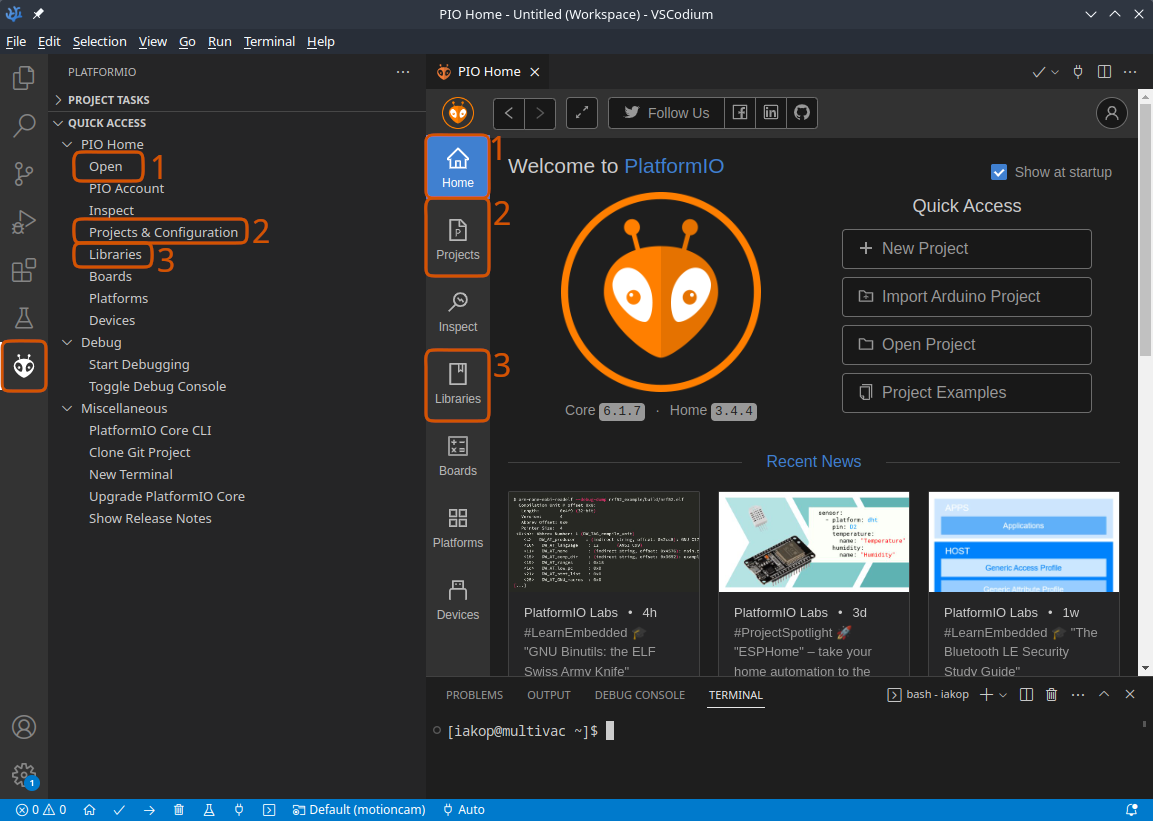
\includegraphics[width=\textwidth,keepaspectratio=true]{assets/pictures/pio-menu.png}
  			\caption{PlatformIO standard view, med \tthigh{Home}, \tthigh{Projects} og \tthigh{Libraries}, samt Quick Access}
  			\label{fig:pio-menu}
		\end{figure}
	\end{column}
	\begin{column}{0.5\textwidth}
		\begin{textBox}
			\begin{itemize}
				\item PlatformIO extensionen kan åbnes ved at klikke på fanen PlatformIO \includesvg[height=12pt, keepaspectratio=true]{assets/svg/pio-logo.svg}
				\item Herunder findes en række muligheder, de vigtigste:
				\begin{enumerate}
					\item Open / Home
					\begin{itemize}
						\item Hovedsiden til PlatformIO, med quick access og faner til resten af funktionerne
					\end{itemize}
					\item Projects \& Configuration \\/ Projects
					\begin{itemize}
						\item Projektside, til at oprette og indstille softwareprojekter
					\end{itemize}
					\item Libraries
					\begin{itemize}
						\item Til søgning og tilføjelse af Libraries til PlatformIO projekter
					\end{itemize}
				\end{enumerate}
			\end{itemize}
		\end{textBox}
	\end{column}
\end{columns}
\end{frame}

\section{Setup af ESP32 projekt i PlatformIO}
\begin{frame}
	\sectiontitle{assets/svg/pio-logo.svg}{\insertsectionhead}
\end{frame}

\begin{frame}{Setup af ESP32 projekt i PlatformIO}
\begin{columns}
	\begin{column}{0.5\textwidth}
		\begin{textBox}
			\begin{itemize}
				\item Klik på fanen \tthigh{Projects} for at få visningen af projekter frem
				\item For at skabe et nyt projekt, klik på \tthigh{Create New Project}
			\end{itemize}
		\end{textBox}
	\end{column}
	\begin{column}{0.5\textwidth}
		\begin{figure}
  			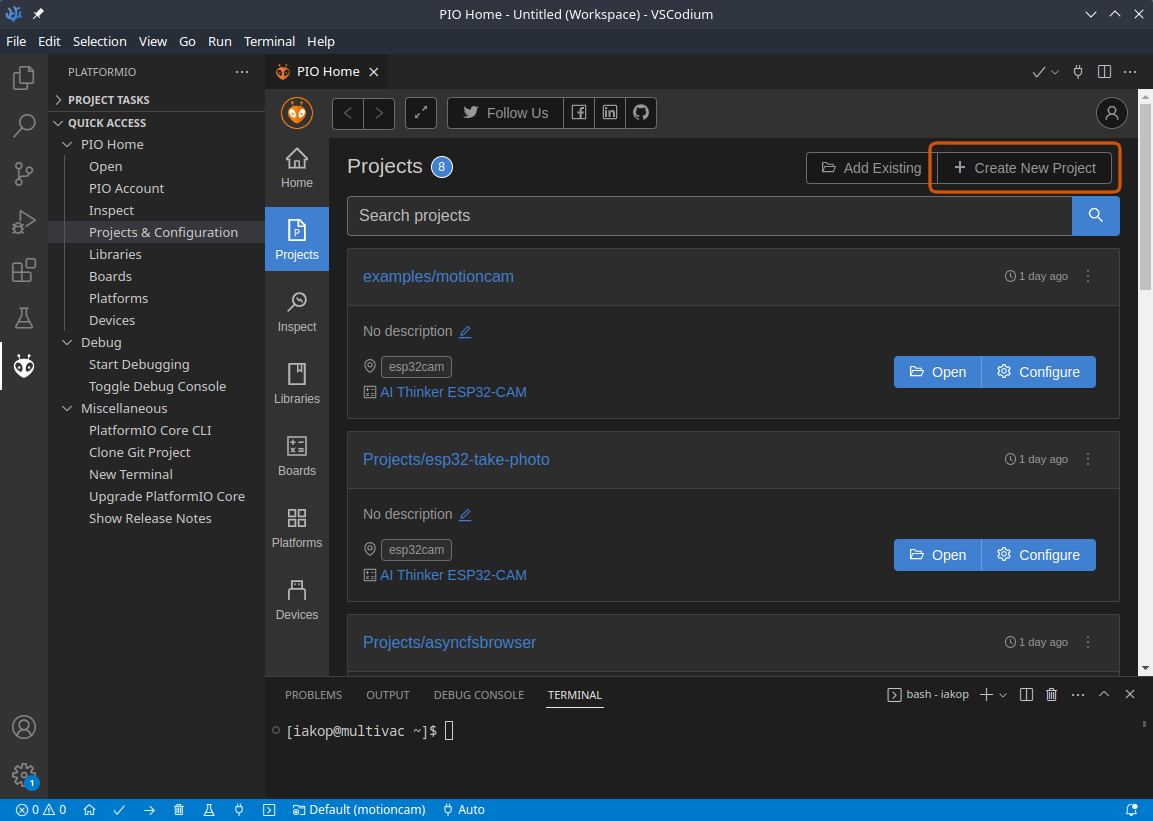
\includegraphics[width=\textwidth,keepaspectratio=true]{assets/pictures/pio-project.png}
  			\caption{\tthigh{Projects} fanen i PlatformIO. Her kan projekter oprettes og redigeres i GUI'en}
  			\label{fig:pio-project}
		\end{figure}
	\end{column}
\end{columns}
\end{frame}

\begin{frame}{Setup af ESP32 projekt i PlatformIO}
\begin{columns}
	\begin{column}{0.5\textwidth}
		\begin{figure}
  			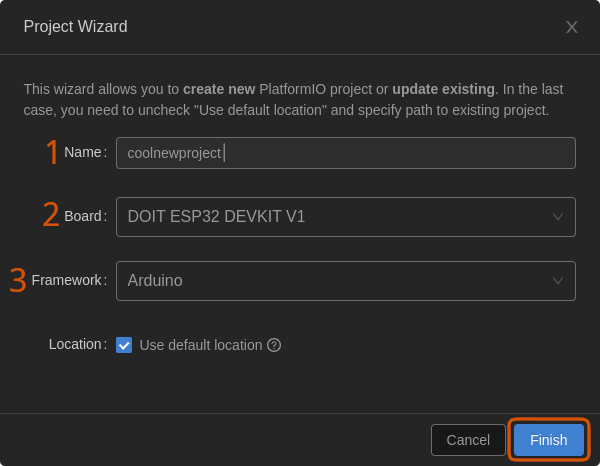
\includegraphics[height=0.7\textheight,keepaspectratio=true]{assets/pictures/pio-project-2.png}
  			\caption{\tthigh{Project Wizard} dialogen i PlatformIO, med indstillinger for navn, board og framework}
  			\label{fig:pio-project2}
		\end{figure}
	\end{column}
	\begin{column}{0.5\textwidth}
		\begin{textBox}
			\begin{itemize}
				\item Der vil komme en \tthigh{Project Wizard} dialog
				\item Den har 3 felter, som i vores tilfælde udfyldes således:
				\begin{itemize}
					\item Name
					\begin{itemize}
						\item Et passende navn til projektet, eks. "\tthigh{coolnewproject}"
					\end{itemize}
					\item Board
					\begin{itemize}
						\item  \tthigh{DOIT ESP32 DEVKIT V1}
					\end{itemize}
					\item Framework
					\begin{itemize}
						\item \tthigh{Arduino}
					\end{itemize}
				\end{itemize}
				\item Afslut ved at trykke \tthigh{Finish}
			\end{itemize}
		\end{textBox}
	\end{column}
\end{columns}
\end{frame}

\begin{frame}{Setup af ESP32 projekt i PlatformIO}
\begin{columns}
	\begin{column}{0.5\textwidth}
		\begin{textBox}
			\begin{itemize}
				\item PlatformIO vil generere et projekt og automatisk sætte værktøjerne op
				\begin{itemize}
					\item Dette kræver en internetforbindelse
				\end{itemize}
				\item Når det er færdigt, indlæses \tthigh{platformio.ini}
				\begin{itemize}
					\item Denne fil indeholder indstillingerne for projektet og kan redigeres i hånden
				\end{itemize}
				\item På siden ses nogle \tthigh{Project Tasks}:
				\begin{enumerate}
					\item Build
					\begin{itemize}
						\item Bygger et image til at programmere hardwaren med
					\end{itemize}
					\item Upload
					\begin{itemize}
						\item Uploader imaget til hardwaren gennem en automatisk detekteret USB/UART forbindelse
					\end{itemize}
					\item Monitor
					\begin{itemize}
						\item Overvåger UART forbindelsen til hardwaren (Baud raten kan indstilles i \tthigh{platformio.ini})
					\end{itemize}
					\item Build Filesystem Image
					\begin{itemize}
						\item Bygger image af et filsystem til hardwaren (ligger i \tthigh{data} mappen under projektet)
						\item \tthigh{data} mappen skal oprettes manuelt
						\item Filsystemet kan specificeres i \tthigh{platformio.ini}
					\end{itemize}
					\item Upload Filesystem Image
					\begin{itemize}
						\item Uploader det byggede filsystem til boardet
						\item \ttwarn{VIGTIGT}: Monitor kan ikke være aktivt under upload
					\end{itemize}
				\end{enumerate}
			\end{itemize}
		\end{textBox}
	\end{column}
	\begin{column}{0.5\textwidth}
		\begin{figure}
  			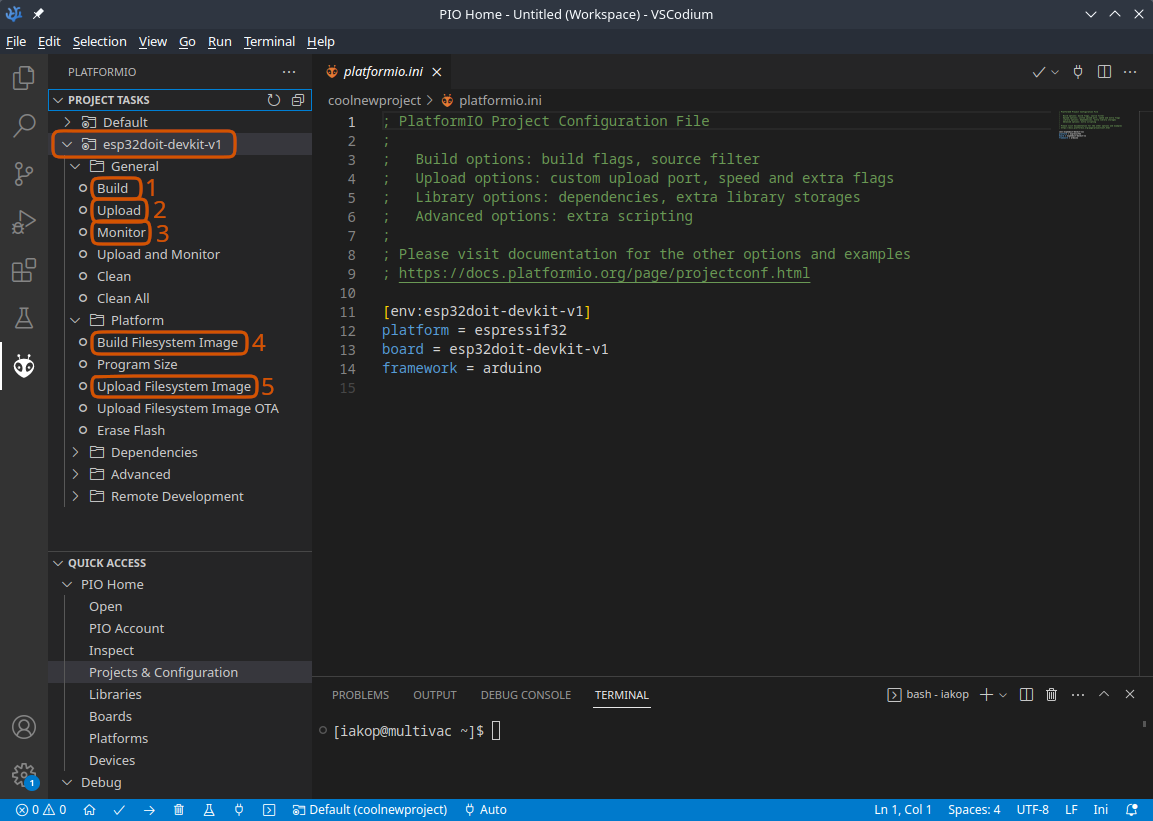
\includegraphics[width=\textwidth,keepaspectratio=true]{assets/pictures/pio-project-3.png}
  			\caption{Åbent projekt i PlatformIO, viser \tthigh{platformio.ini} samt hvilke \tthigh{Project Tasks} der er mulige for projektet}
  			\label{fig:pio-project3}
		\end{figure}
	\end{column}
\end{columns}
\end{frame}

\subsection{Tilføj libraries til ESP32 projekt}
\begin{frame}{Tilføj libraries til ESP32 projekt}
\begin{columns}
	\begin{column}{0.5\textwidth}
		\begin{figure}
  			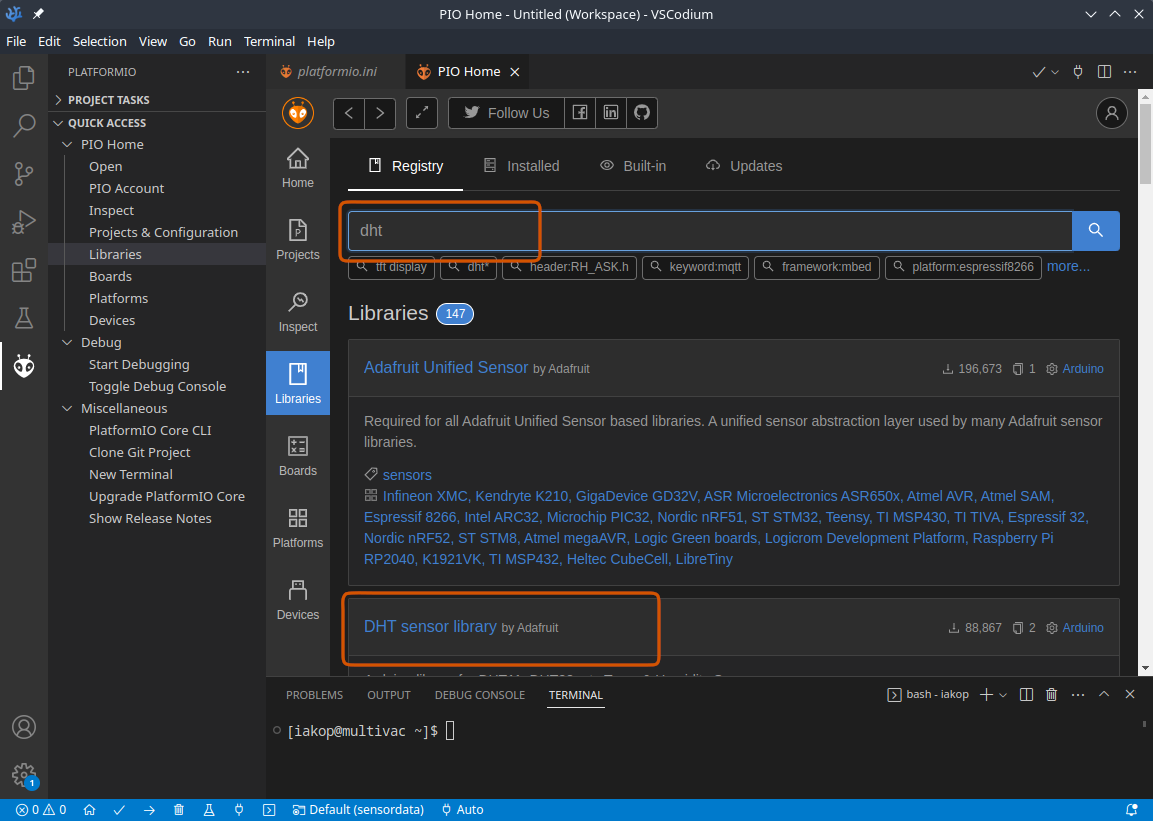
\includegraphics[width=\textwidth,keepaspectratio=true]{assets/pictures/pio-libraries.png}
  			\caption{\tthigh{Libraries} fanen i PlatformIO. Her kan libraries søges frem og tilføjes til projekter}
  			\label{fig:pio-libraries}
		\end{figure}
	\end{column}
	\begin{column}{0.5\textwidth}
		\begin{textBox}
			\begin{itemize}
				\item For at tilføje eksterne libraries til ens projekt, kan man man under \tthigh{Libraries} fanen søge efter libraries
				\begin{itemize}
					\item De kan fremsøges under \tthigh{Registry}
					\item Installerede libraries kan vises under \tthigh{Installed}
				\end{itemize}
				\item Herefter klik på det relevante library
			\end{itemize}
		\end{textBox}
	\end{column}
\end{columns}
\end{frame}

\begin{frame}{Tilføj libraries til ESP32 projekt}
\begin{columns}
	\begin{column}{0.5\textwidth}
		\begin{textBox}
			\begin{itemize}
				\item Inde under det pågældende library kan der findes:
				\begin{itemize}
					\item Eksempler
					\item Headers
					\item mm.
				\end{itemize}
				\item Klik \tthigh{Add to Project} for at tilføje den til et projekt
			\end{itemize}
		\end{textBox}
	\end{column}
	\begin{column}{0.5\textwidth}
		\begin{figure}
  			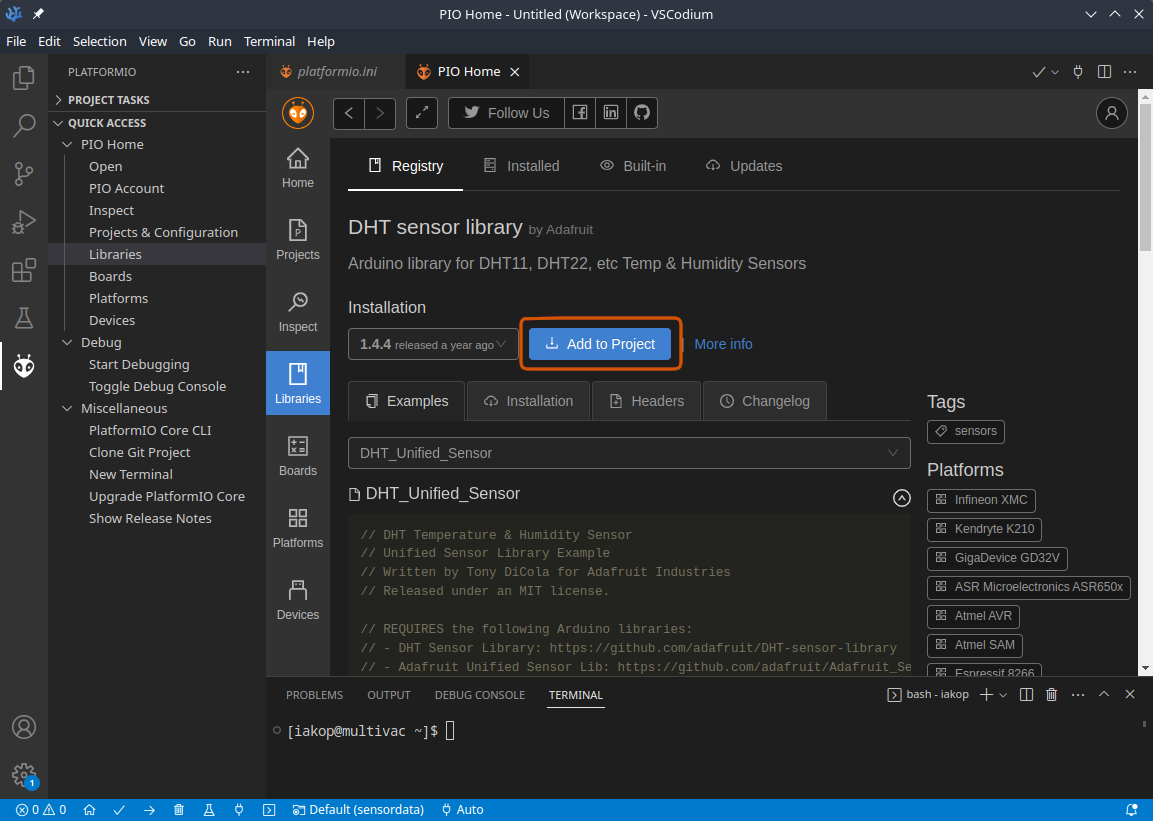
\includegraphics[width=\textwidth,keepaspectratio=true]{assets/pictures/pio-libraries-2.png}
  			\caption{\tthigh{DHT sensor library} i PlatformIO. Kan tilføjes til projekter, og understøtter Arduino frameworket}
  			\label{fig:pio-libraries-2}
		\end{figure}
	\end{column}
\end{columns}
\end{frame}

\begin{frame}{Tilføj libraries til ESP32 projekt}
\begin{columns}
	\begin{column}{0.5\textwidth}
		\begin{figure}
  			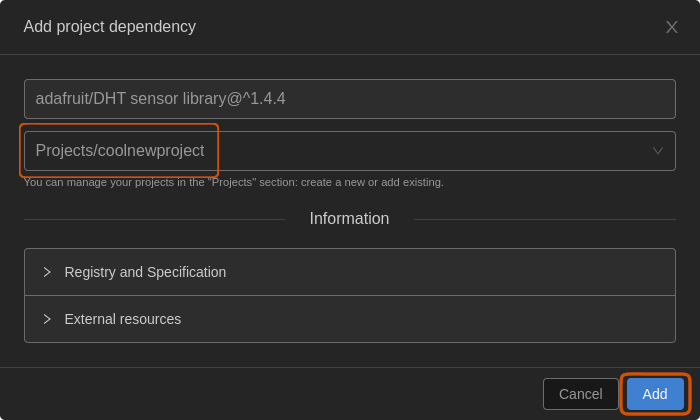
\includegraphics[width=\textwidth,keepaspectratio=true]{assets/pictures/pio-libraries-3.png}
  			\caption{\tthigh{Add project dependency} dialogen i PlatformIO. Har vælges hvilket projekt der skal tilføjes et library}
  			\label{fig:pio-libraries-3}
		\end{figure}
	\end{column}
	\begin{column}{0.5\textwidth}
		\begin{textBox}
			\begin{itemize}
				\item Der åbnes en \tthigh{Add project dependency} dialog
				\item Vælg under \tthigh{Select a project}, hvilket projekt der skal bruge librariet
				\item Klik \tthigh{Add}
				\item PlatformIO tilføjer automatisk en \tthigh{lib\_deps} dependency i \tthigh{platformio.ini}, og sætter librariet op
			\end{itemize}
		\end{textBox}
	\end{column}
\end{columns}
\end{frame}

\subsection{Indlæsning af ESP32 Projekt i PlatformIO}
\begin{frame}{Indlæsning af ESP32 Projekt i PlatformIO}
\begin{columns}
	\begin{column}{0.5\textwidth}
		\begin{figure}
  			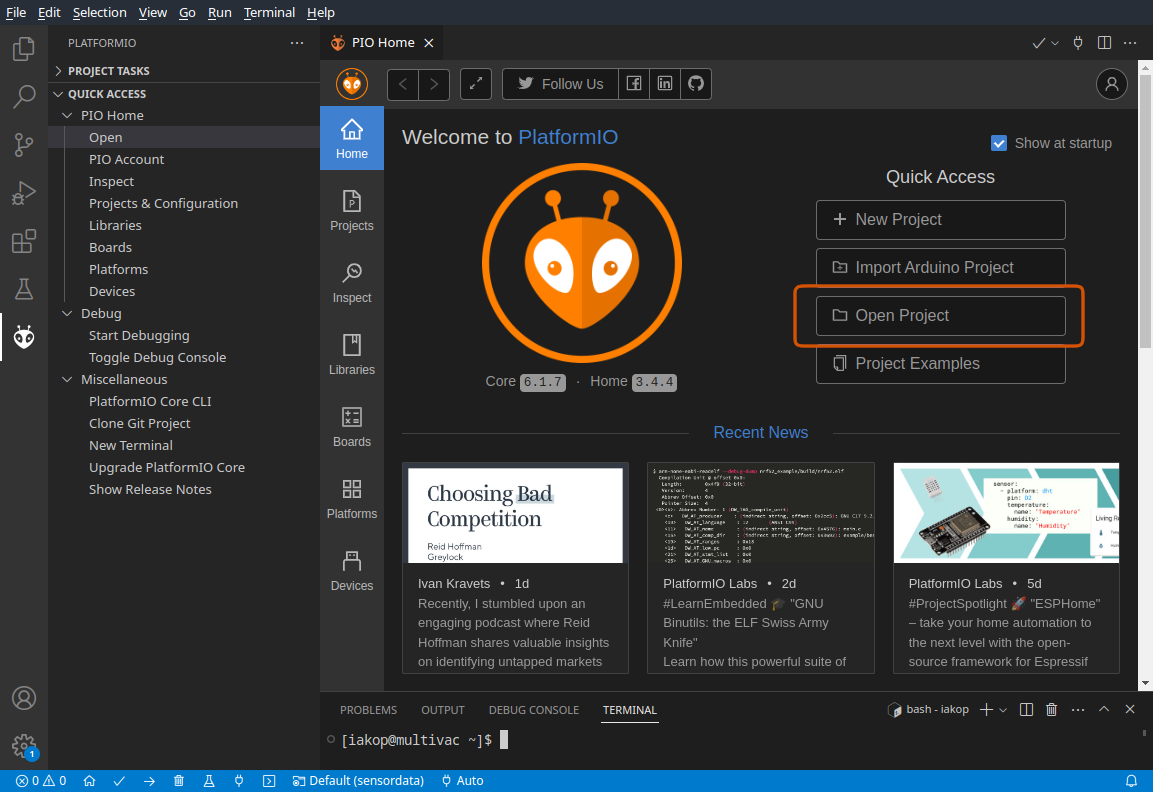
\includegraphics[width=\textwidth,keepaspectratio=true]{assets/pictures/pio-import.png}
  			\caption{\tthigh{Home} fanen i PlatformIO, med markeret indstilling for at indlæse et projekt fra disk}
  			\label{fig:pio-project4}
		\end{figure}
	\end{column}
	\begin{column}{0.5\textwidth}
		\begin{textBox}
			\begin{itemize}
				\item Projekterne i denne workshop bruger specifikke libraries og indstillinger
				\item For at have dem sat op hurtigt, kan hele projekter indlæses fra Github repoet
				\item Download hele workshoppens materialer her:
				\begin{itemize}
					\item \small\url{https://github.com/iakop/IoT-Crashcourse/archive/refs/heads/master.zip}
				\end{itemize}
				\item Pak dem ud hvor de kan findes
				\item Under \tthigh{Home} fanen, klik \tthigh{Open Project}
			\end{itemize}
		\end{textBox}
	\end{column}
\end{columns}
\end{frame}

\begin{frame}{Indlæsning af ESP32 Projekt i PlatformIO}
\begin{columns}
	\begin{column}{0.5\textwidth}
		\begin{textBox}
			\begin{itemize}
				\item I \tthigh{Open PlatformIO Project} dialogen, åbn mappen hvor eksemplerne ligger
				\item Hvis \tthigh{Open} knappen f.eks. siger \tthigh{Open "simpleServer"} står dialogen det rigtige sted
				\item Klik \tthigh{Open} knappen
			\end{itemize}
		\end{textBox}
	\end{column}
	\begin{column}{0.5\textwidth}
		\begin{figure}
  			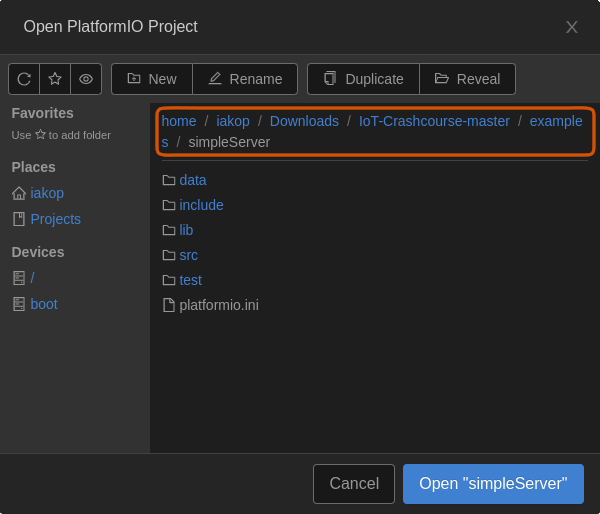
\includegraphics[height=0.7\textheight,keepaspectratio=true]{assets/pictures/pio-project-5.png}
  			\caption{\tthigh{Open PlatformIO Project} dialogen i PlatformIO. For at åbne et projekt, skal man finde den på disken, og stå i mappen e.g.: \tthigh{Downloads/IoT-Crashcourse-master/examples/simpleServer}}
  			\label{fig:pio-project5}
		\end{figure}
	\end{column}
\end{columns}
\end{frame}

\begin{frame}{Indlæsning af ESP32 Projekt i PlatformIO}
\begin{columns}
	\begin{column}{0.5\textwidth}
		\begin{figure}
  			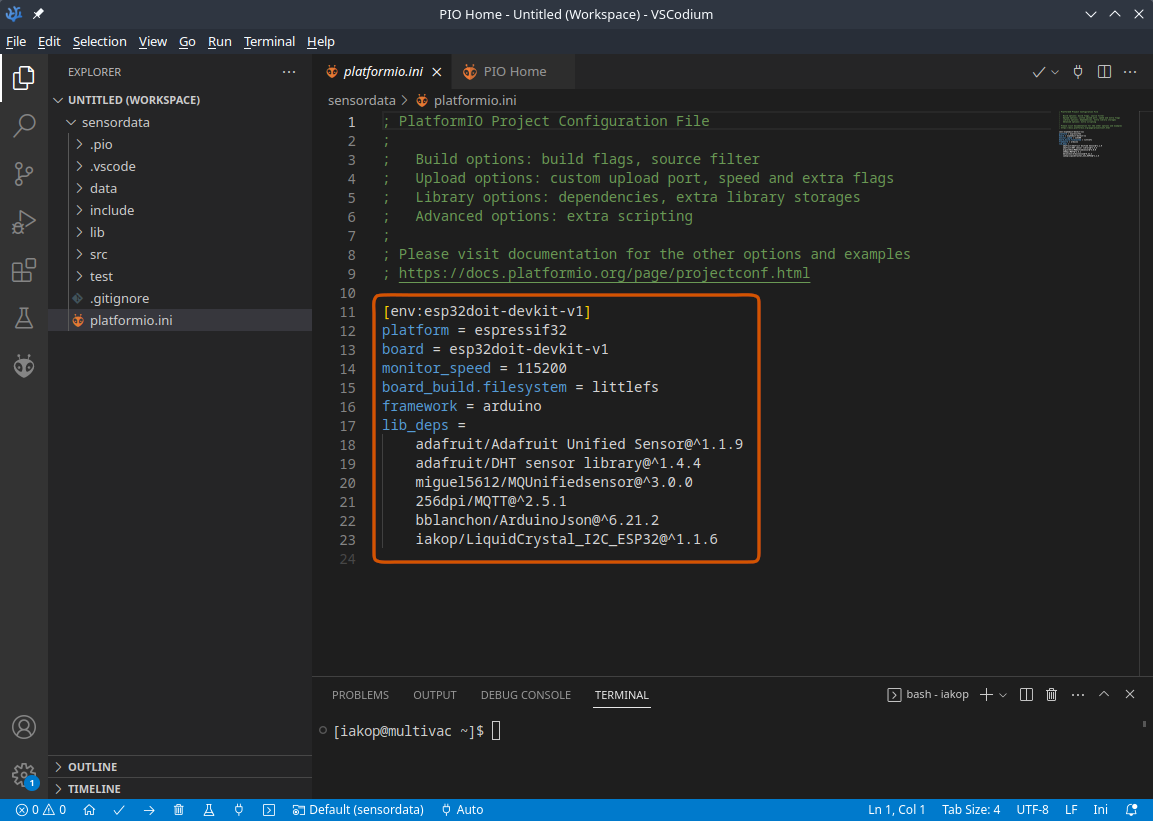
\includegraphics[width=\textwidth,keepaspectratio=true]{assets/pictures/pio-projects-6.png}
  			\caption{Eksempel på et \tthigh{platformio.ini} for et projekt. Bemærk \tthigh{monitor-speed}, \tthigh{filesystem} og \tthigh{lib\_deps} er defineret}
  			\label{fig:pio-project6}
		\end{figure}
	\end{column}
	\begin{column}{0.5\textwidth}
		\begin{textBox}
			\begin{itemize}
				\item Når projektet er indlæst, åben \tthigh{platformio.ini} for projektet
				\item Den specificerer alle libraries og komponenter projektet afhænger af
				\item Værktøjerne og indstillingerne for projektet sættes automatisk op af PlatformIO
			\end{itemize}
		\end{textBox}
	\end{column}
\end{columns}
\end{frame}

\section{IoT basics}
\begin{frame}
	\sectiontitle{assets/svg/iot-star.svg}{\insertsectionhead}
\end{frame}

\begin{frame}{IoT basics}
\begin{columns}
	\begin{column}{0.6\textwidth}
		\begin{textBox}
			\begin{itemize}
				\item IoT (Internet of Things), er en fællesbetegnelse for netværksopkoblede genstande
				\item En sådan genstand indeholder typisk:
				\begin{itemize}
					\item En microprocessor eller -computer
					\item Sensorer
					\item Aktuatorer
					\item Trådet eller trådløs opkobling
				\end{itemize}
			\end{itemize}
		\end{textBox}
	\end{column}
	\begin{column}{0.4\textwidth}
		\centering
		\begin{figure}
			\captionsetup{format=tcbcaptionminmargin}
			\roundedGfx{0.9\textwidth}{assets/pictures/nedis-smartplug.jpg}
  			\caption{Nedis SmartLife adskilt for at komme til indmaden. Indeholder bla. et TYWE3S WiFi modul og en HLW8012 effektsensor
  			\captionline \textbf{Kilde:} \url{https://callaa.github.io/2021/01/26/liberating-nedis-smartplug.html}}
  			%\caption{Nedis SmartLife adskilt for at komme til indmaden. Indeholder bla. et TYWE3S WiFi modul og en HLW8012 effektsensor}
  			\label{fig:iot-device}
		\end{figure}
	\end{column}
\end{columns}
\end{frame}

\begin{frame}{IoT basics}
\begin{columns}
	\begin{column}{0.5\textwidth}
		\centering
		\captionsetup{format=tcbcaptionsmall}
		\begin{columns}
			\begin{column}{0.5\textwidth}
				\begin{figure}[height=0.2\textheight]
  					\includesvg[height=0.2\textheight]{assets/svg/iot-star.svg}
  					\caption{Star-topologi, hvor hver enhed kommunikerer med en central gateway til resten af internettet}
  					\label{fig:iot-star}
				\end{figure}
			\end{column}
			\begin{column}{0.5\textwidth}
				\begin{figure}[height=0.2\textheight]
  					\includesvg[height=0.2\textheight]{assets/svg/iot-tree.svg}
  					\caption{Tree-topologi, hvor enhederne er forbundet i forgreninger, og videregiver informationer herigennem til gateway}
  					\label{fig:iot-tree}
				\end{figure}
			\end{column}
		\end{columns}
		\begin{columns}
			\begin{column}{0.5\textwidth}
				\begin{figure}[height=0.2\textheight]
  					\includesvg[height=0.2\textheight]{assets/svg/iot-mesh.svg}
  					\caption{Mesh-topologi, hvor alle enheder kommunikerer internt, og videre giver information gennem hinanden til gateway}
  					\label{fig:iot-mesh}
				\end{figure}
			\end{column}
		\end{columns}
	\end{column}
	\begin{column}{0.5\textwidth}
		\begin{textBox}
			\begin{itemize}
				\item Kommunikation mellem enheder foregår på mange forskellige måder
				\item Nogle gængse netværkstopologier er bla.:
				\begin{itemize}
					\item Star
					\item Tree
					\item Mesh
				\end{itemize}
			\end{itemize}
		\end{textBox}
	\end{column}
\end{columns}
\end{frame}

\begin{frame}{IoT basics}
\begin{columns}
	\begin{column}{0.6\textwidth}
		\begin{textBox}
			\begin{itemize}
				\item Der findes en række protokoller for enheder at kommunikere gennem
				\item Dem vi vil fokusere på:
				\begin{itemize}
					\item HTTP
						\begin{itemize}
							\item Den gængse Hypertext Transfer Protocol, der bruges til at overføre webindhold, bla. mellem servere og browsere
						\end{itemize}
					\item WebSocket
						\begin{itemize}
							\item En fuld duplex (tovejs kommunikation) protokol til hurtig samtidig kommunikation mellem klient og server - lav overhead
						\end{itemize}
					\item MQTT
						\begin{itemize}
							\item (Oprindeligt forkortelse for MQ (Message Queue) Telemetry Transport) Publish-subscribe baseret protokol mellem enheder og central broker - lav overhead
						\end{itemize}
				\end{itemize}
			\end{itemize}
		\end{textBox}
	\end{column}
	\begin{column}{0.4\textwidth}
		\centering
		\captionsetup{format=tcbcaptionsmall}
		\begin{columns}
			\begin{column}{0.45\textwidth}
				\begin{figure}[height=0.2\textheight]
  					\includesvg[height=0.2\textheight]{assets/svg/http-logo.svg}
  					\caption{HTTP logo
  					\captionline \textbf{Kilde:} \url{https://en.wikipedia.org/wiki/File:HTTP_logo.svg}
  					\captionline \textbf{Licens:} Public Domain}
  					\label{fig:http-logo}
				\end{figure}
			\end{column}
			\begin{column}{0.45\textwidth}
				\begin{figure}[height=0.2\textheight]
  					\includesvg[height=0.2\textheight]{assets/svg/websocket-logo.svg}
  					\caption{WebSocket logo
  					\captionline \textbf{Kilde:} \url{https://logodix.com/logos/1825947}
  					\captionline \textbf{Licens:} Non-Commercial}
  					\label{fig:websocket-logo}
				\end{figure}
			\end{column}
		\end{columns}
		\begin{columns}
			\begin{column}{0.45\textwidth}
				\begin{figure}[height=0.2\textheight]
  					\includesvg[height=0.2\textheight]{assets/svg/mqtt-logo.svg}
  					\caption{MQTT logo
  					\captionline \textbf{Kilde:} \url{https://en.wikipedia.org/wiki/File:Mqtt-hor.svg}
  					\captionline \textbf{Licens:} Public Domain}
  					\label{fig:mqtt-logo}
				\end{figure}
			\end{column}
		\end{columns}
	\end{column}
\end{columns}
\end{frame}

\section{Byg en simpel ESP32 webserver}
\begin{frame}
	\sectiontitle{assets/pictures/simpleserver.png}{\insertsectionhead}
\end{frame}

\subsection{Eksempel: Simpel Server}
\begin{frame}{Simpel Server}
\begin{columns}
	\begin{column}{0.6\textwidth}
		\begin{textBox}
		\begin{itemize}
			\item Til vores eksempel skal vi bruge en breadboard opstilling
			\begin{itemize}
				\item Et ESP32 board
				\item En LED
				\item En 220{\textsf{$\Omega$}} modstand
			\end{itemize}
			\item HTML og Arduino programmet gennemgår vi i fællesskab
			%\captionbreak
			\item Kildefiler kan hentes på:
			\begin{itemize}
				\item \tiny\url{https://github.com/iakop/IoT-Crashcourse/tree/master/examples/simpleServer}
			\end{itemize}
		\end{itemize}
		\end{textBox}
	\end{column}
	\begin{column}{0.4\textwidth}
		\centering
		\begin{figure}
  			\includesvg[height=0.6\textheight]{assets/setups/esp32-led.svg}
  			\caption{Breadboard setup med ESP32 og LED}
  			\label{fig:esp32-led}
		\end{figure}
	\end{column}
\end{columns}
\end{frame}

\section{WebSockets på ESP32}
\begin{frame}
	\sectiontitle{assets/pictures/websocketserver.png}{\insertsectionhead}
\end{frame}

\subsection{Eksempel: WebSocket Server}
\begin{frame}{WebSocket Server}
\begin{columns}
	\begin{column}{0.6\textwidth}
		\begin{textBox}
		\begin{itemize}
			\item Til dette eksempel tilføjes en sensor til vores opstilling
			\begin{itemize}
				\item Et ESP32 board
				\item En LED
				\item En 220{\textsf{$\Omega$}} modstand
				\item Et DHT11 temperatur-/fugtighedssensor modul
			\end{itemize}
			\item Der skal tilføjes Javascript og WebSocket forbindelse, som vi gennemgår i fællesskab
			\item Kildefiler kan hentes på:
			\begin{itemize}
				\item \tiny\url{https://github.com/iakop/IoT-Crashcourse/tree/master/examples/websocketServer}
			\end{itemize}
		\end{itemize}
		\end{textBox}
	\end{column}
	\begin{column}{0.4\textwidth}
		\centering
		\begin{figure}
  			\includesvg[height=0.6\textheight]{assets/setups/esp32-led-dht11.svg}
  			\caption{Breadboard setup med ESP32, LED og DHT11 sensor}
  			\label{fig:esp32-led-dht11}
		\end{figure}
	\end{column}
\end{columns}
\end{frame}

\section{MQTT på ESP32}
\begin{frame}
	\sectiontitle{assets/pictures/mqttclient.png}{\insertsectionhead}
\end{frame}

\subsection{Eksempel: MQTT Client}
\begin{frame}{MQTT Client}
\begin{columns}
	\begin{column}{0.6\textwidth}
		\begin{textBox}
		\begin{itemize}
			\item Samme opstilling som sidst
			\begin{itemize}
				\item Et ESP32 board
				\item En LED
				\item En 220{\textsf{$\Omega$}} modstand
				\item Et DHT11 temperatur-/fugtighedssensor modul
			\end{itemize}
			\item Al server kode skiftes ud med client kode, som forbinder via SSL til en hosted MQTT broker
			\item Kildefiler kan hentes på:
			\begin{itemize}
				\item \tiny\url{https://github.com/iakop/IoT-Crashcourse/tree/master/examples/mqttClient}
			\end{itemize}
		\end{itemize}
		\end{textBox}
	\end{column}
	\begin{column}{0.4\textwidth}
		\centering
		\begin{figure}
  			\includesvg[height=0.6\textheight]{assets/setups/esp32-led-dht11.svg}
  			\caption{Breadboard setup med ESP32, LED og DHT11 sensor}
  			\label{fig:esp32-led-dht11-2}
		\end{figure}
	\end{column}
\end{columns}
\end{frame}

\begin{frame}{MQTT Client}
\begin{columns}
\begin{column}{0.6\textwidth}
		\centering
		\begin{figure}
  			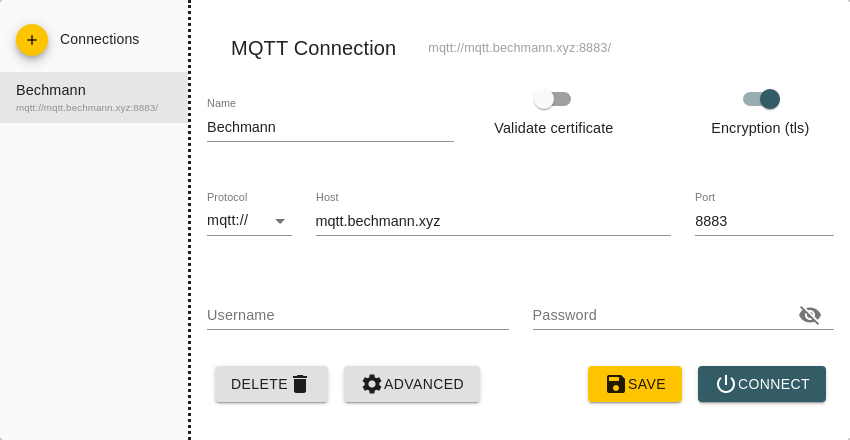
\includegraphics[width=\textwidth]{assets/pictures/mqtt-explorer.png}
  			\caption{MQTT Explorer Connection dialogvindue, her med forbindelsen til \tthigh{mqtt.bechmann.xyz} defineret}
  			\label{fig:mqtt-explorer}
		\end{figure}
	\end{column}
	\begin{column}{0.4\textwidth}
		\begin{textBox}
		\begin{itemize}
			\item MQTT Explorer kan bruges til at tjekke topics:
			\begin{itemize}
				\item \small\url{http://mqtt-explorer.com/}
			\end{itemize}
			\item Indstillinger for forbindelse til workshoppens \ttwarn{offentlige} server:
			\begin{itemize}
				\item Name: \tthigh{Bechmann} (Valgfri)	
				\item Validate certificate:	 \tthigh{off} 
				\begin{itemize}
					\item \ttlow{Bug i MQTT Explorers cert storage forhindrer validering}
				\end{itemize}
				\item Encryption (tls):	 \tthigh{on} 
				\item Protocol: \tthigh{mqtt://}
				\item Host: \tthigh{mqtt.bechmann.xyz}
				\item Port: \tthigh{8883}
				\item Username: \ttlow{blank}
				\item Password: \ttlow{blank}
			\end{itemize}
		\end{itemize}
		\end{textBox}
	\end{column}
\end{columns}
\end{frame}

\end{document}